% Compact horizontal architecture figure for the poster. Natural width 12 cm; smallest text 7.2 pt when scaled to 12 cm (natural width 12.2 cm, small text 7.3 pt).
% Build: bash docs/assets/build.sh compact
\documentclass[11pt,border=0.3pt]{standalone}
\usepackage{times}
\usepackage[T1]{fontenc}
\usepackage[utf8]{inputenc}
\usepackage{xcolor}
\usepackage{tikz}
\usetikzlibrary{positioning,fit,backgrounds,arrows.meta,calc}
\definecolor{locF}{HTML}{E3F1E0}\definecolor{locD}{HTML}{4E7D46}
\definecolor{modF}{HTML}{DDEAF6}\definecolor{modD}{HTML}{2F5D8A}
\definecolor{gtF}{HTML}{FCEBD0}\definecolor{gtD}{HTML}{A8690B}
\definecolor{psF}{HTML}{F7DADA}\definecolor{psD}{HTML}{A23B3B}
\definecolor{stF}{HTML}{ECE6F5}\definecolor{stD}{HTML}{6A5293}
\definecolor{lgF}{HTML}{EFEFEF}
\newcommand{\sm}[1]{{\fontsize{7.3}{8.3}\selectfont #1}}
\begin{document}
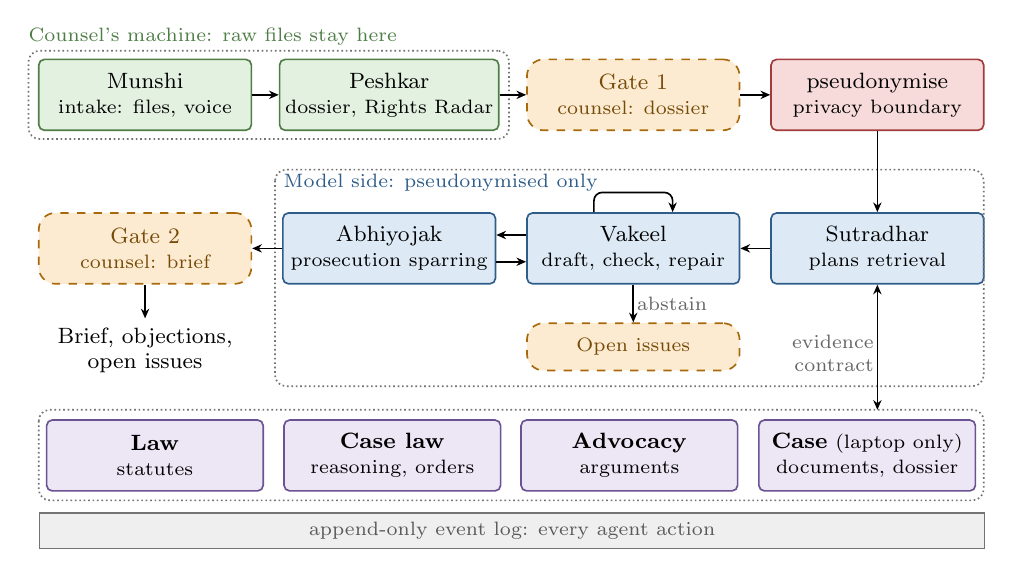
\begin{tikzpicture}[
  font=\fontsize{8}{9}\selectfont, >={Stealth[length=3.5pt,width=3pt]}, line width=0.6pt,
  ag/.style={draw=modD, fill=modF, rounded corners=2pt, align=center, minimum width=2.7cm, minimum height=0.9cm, inner sep=2pt},
  loc/.style={ag, draw=locD, fill=locF},
  gt/.style={ag, draw=gtD, fill=gtF, text=gtD!70!black, dashed, rounded corners=6pt},
  sh/.style={draw=stD, fill=stF, rounded corners=2pt, align=center, minimum width=2.75cm, minimum height=0.9cm, inner sep=2pt},
  lb/.style={font=\fontsize{7.3}{8.3}\selectfont, text=black!60, align=left, inner sep=1pt},
  fr/.style={draw=black!55, densely dotted, rounded corners=4pt}]
% columns x = 1.35, 4.45, 7.55, 10.65 ; rows y = 0, -1.95, -3.2
\node[loc] (mu) at (1.35,0) {Munshi\\\sm{intake: files, voice}};
\node[loc] (pe) at (4.45,0) {Peshkar\\\sm{dossier, Rights Radar}};
\node[gt]  (g1) at (7.55,0) {Gate 1\\\sm{counsel: dossier}};
\node[draw=psD, fill=psF, rounded corners=2pt, minimum width=2.7cm, minimum height=0.9cm, align=center, inner sep=2pt] (ps) at (10.65,0) {pseudonymise\\\sm{privacy boundary}};
\node[gt]  (g2) at (1.35,-1.95) {Gate 2\\\sm{counsel: brief}};
\node[ag]  (ab) at (4.45,-1.95) {Abhiyojak\\\sm{prosecution sparring}};
\node[ag]  (va) at (7.55,-1.95) {Vakeel\\\sm{draft, check, repair}};
\node[ag]  (su) at (10.65,-1.95) {Sutradhar\\\sm{plans retrieval}};
\node[align=center, minimum width=2.7cm] (out) at (1.35,-3.25) {Brief, objections,\\open issues};
\node[gt, minimum height=0.6cm] (oi) at (7.55,-3.2) {\sm{Open issues}};
% frames
\node[fr, fit=(mu)(pe), inner xsep=0.12cm, inner ysep=0.1cm] (lap) {};
\node[lb, anchor=south west, text=locD, inner sep=0pt] at ([yshift=1.5pt]lap.north west) {Counsel's machine: raw files stay here};
\draw[fr] (3.0,-0.95) rectangle (12.0,-3.7);
\node[lb, anchor=north west, text=modD, inner sep=0pt] at (3.1,-1.0) {Model side: pseudonymised only};
% stores
\draw[fr] (0,-4.0) rectangle (12.0,-5.15);
\foreach \i/\x in {1/1.475,2/4.49,3/7.5,4/10.52}
  \coordinate (c\i) at (\x,-4.58);
\node[sh] at (c1) {\textbf{Law}\\\sm{statutes}};
\node[sh] at (c2) {\textbf{Case law}\\\sm{reasoning, orders}};
\node[sh] at (c3) {\textbf{Advocacy}\\\sm{arguments}};
\node[sh] at (c4) {\textbf{Case} \sm{(laptop only)}\\\sm{documents, dossier}};
\node[draw=black!55, fill=lgF, minimum width=12cm, minimum height=0.45cm, anchor=north west, inner sep=0pt, text=black!65] (lg) at (0,-5.3) {\sm{append-only event log: every agent action}};
% flow
\draw[->] (mu) -- (pe);
\draw[->] (pe) -- (g1);
\draw[->] (g1) -- (ps);
\draw[->] (ps) -- (su);
\draw[->] (su) -- (va);
\draw[->] ($(va.west)+(0,0.17)$) -- ($(ab.east)+(0,0.17)$);
\draw[->] ($(ab.east)+(0,-0.17)$) -- ($(va.west)+(0,-0.17)$);
\draw[->] (ab) -- (g2);
\draw[->] (g2) -- (out);
\draw[->, rounded corners=3pt] ($(va.north)+(-0.5,0)$) -- ++(0,0.25) -- ++(1.0,0) -- ($(va.north)+(0.5,0)$);
\draw[->] (va) -- node[lb, right] {abstain} (oi);
\draw[<->] (su) -- node[lb, left, align=right, pos=0.55] {evidence\\contract} (10.65,-4.0);
\end{tikzpicture}
\end{document}
